\section{Design Principles 1}
\section{Part I: Dimensions of Software Quality}
\subsection{Software Quality}
\begin{defBox}[title=How to assure software quality? The big picture]
    Define a \red{quality assurance (QA) plan} (\enquote{\blue{Plan zur Qualitätssicherung}}) (must be integrated into the software development process)
    \begin{itemize}
        \item Constatly \red{assess} design \red{quality} (quantitative, qualitative)
        \item Be proficient in applying time-tested \red{design principles}
        \item Use tools and \red{design techniques} that help to achieve quality 
        \item Use \red{design patterns} to learn from and reuse proven slutions to recurring problems
        \item Systematically \red{verify} correctness \& performance of design 
        \item\red{Validate} fulfillment of requirements
    \end{itemize}
\end{defBox}
\begin{infoBox}
    \begin{enumerate}
        \item \fatsf{QA-Plan definieren}
        \begin{itemize}
            \item A \fatsf{Qualitätssicherungsplan (QA) plan} ist unverzichtbar und muss in den Softwareentwicklungsprozess integriert werden. Der Plan beschreibt Aktivitäten , Zeitplänne, Werkzeuge und Rollen, um die Qulität während des gesamten Entwicklungsprozesses sicherzustellen.
        \end{itemize}
        \item \fatsf{Designqualität kontinuierlich bewerten}
        \begin{itemize}
            \item Das Design sollte regelmäßíg anhand \fatsf{quantitativer} (z.B. Metriken) und \fatsf{qualitativer} (z.B. Expertenbewertungen) Methoden überprüft werden, um Probleme frühzeitig zu erkennen und zu beheben.
        \end{itemize}
        \item \fatsf{Bewährte Designprinzipien anwenden}
        \begin{itemize}
            \item Durch die Einhaltung bewährter \fatsf{Designprinzipien} (z.B. SOLID, DRY, KISS) wird sichergestellt, dass die Software robust und wartbar bleibt.
        \end{itemize}
        \item \fatsf{Nutzung von Werkzeugen und Techniken}
        \begin{itemize}
            \item Verwenden Sie Tools (z.B. statische Code-Analyse, CI/CD-Pipelines) und Techniken (z.B. testgetriebene Entwicklung, Paarprogrammierung), die den Entwicklungsprozess effizienter und qualitativ hochwertiger machen.
        \end{itemize}
        \item \fatsf{Design Patterns einsetzen}
        \begin{itemize}
            \item \fatsf{Design Patterns} bieten wiederverwendbare, bewährte Lösungen für häufig auftretende Probleme und minimieren Fehlerquellen.
        \end{itemize}
        \item \fatsf{Korrektheit und Leistung überprüfen}
        \begin{itemize}
            \item Systematische Überprüfungsmethoden wie Tests (Unit-, Integrations-, und Systemtests) oder Performance-Analysen helfen sicherzustellen, dass das Design die Anforderungen erfüllt.
        \end{itemize}
        \item \fatsf{Erfüllung der Anforderungen validieren}
        \begin{itemize}
            \item Die entwickelte Software sollte fortlaufend mit den definierten Anforderungen abgeglichen werden, um sicherzustellen, dass sie die vorgesehenen Funktionalitäten und Leistungsziele erreicht.
        \end{itemize}
    \end{enumerate}
\end{infoBox}

\subsection{Internal and External Quality Factors}
\begin{defBox}[title=What is good software?]
    \red{Internal quality factors} - Perceivable only by computer professionals
    \begin{itemize}
        \item \blue{White box} view of a software system
    \end{itemize}
    \red{External quality factors} - Perceived by the customer \/ user
    \begin{itemize}
        \item \blue{Black box} view of a softare system
        \item Depend on internal quality factors
    \end{itemize}
\end{defBox}
\begin{infoBox}[title=Was ist gute Software?]
    Gute Software zeichnet sich durch interne und externe Qualitätsfaktoren aus, die verschiedene Perspektiven auf die Qualität eines Softwaresystems bieten:
\end{infoBox}
\begin{infoBox}[title=Interne Qualitätsfaktoren]
    \begin{itemize}
        \item \fatsf{Definition:} Aspekte, die nur von Computerprofis (Entwicklern, Architekten) whargenommen werden können.
        \item \fatsf{Whitebox-Perspektie:} Betrachtung des inneren Aufbaus der Software, z.B. des Codes und der Architektur
        \item \fatsf{Beispiele:}
        \begin{itemize}
            \item \fatsf{Wartbarkeit:} Wie leicht kann der Code verändert oder erweitert werden?
            \item \fatsf{Lesbarkeit:} Ist der Code verständlich und klar strukturiert?
            \item \fatsf{Modularität:} Ist die Software in sinnvolle Einheiten zerlegt?
            \item \fatsf{Fehlerfreiheit:} Sind interne Fehlerquellen minimiert?
        \end{itemize}
    \end{itemize}
\end{infoBox}
\begin{infoBox}[title=Externe Qualitätsfaktoren]
    \begin{itemize}
        \item \fatsf{Definition:} Eigenschaften, die direkt von Kunden oder Endnutzern whargenommen werden.
        \item \fatsf{Blackbox-Perspektive:} Fokus auf die Funktionalität und Leistung der Software, ohne die interne Struktur zu kennen.
        \item \fatsf{Beispiele:}
        \begin{itemize}
            \item \fatsf{Benutzerfreundlichkeit:} Ist die Software intuitiv und leicht zu bedienen?
            \item \fatsf{Zuverlässigkeit:} Funktioniert die Software stabil und fehlerfrei?
            \item \fatsf{Leistung (Performance):} Läuft die Software effizient und schnell?
            \item \fatsf{Sicherheit:} Schützt die Software vor unberechtigtem Zugriff und Datenverlust?
        \end{itemize}
    \end{itemize}
\end{infoBox}
\subsection{Software Quality: Internal Factors}
\begin{defBox}[title=Some important internal quality factors]
    \begin{itemize}
        \item \red{Modularity}
        \item \red{Comprehensibility} (\enquote{\blue{Verständlichkeit}}), not overly complex
        \item \red{Cohesion:} clear responsibilities
        \item \red{Concision} (\enquote{\blue{Prägnanz}}): little code duplication, clear code
        \item \red{Correctness}
    \end{itemize}
\end{defBox}
\begin{defBox}
    We will talk about how to judge and how to ensure these quality factors
\end{defBox}
\subsection{Software Quality: External Factors}
\begin{defBox}[title=External quality facotrs\, perceived by Costomer or User]
    \begin{itemize}
        \item \fatsf{Validity:} The ability of software to perform as defined in its requirements
        \begin{itemize}
            \item \red{Precise requirements} definition is needed
            \item Validity depends on correct \red{design}
            \item Validity is often \red{conditional} to correctness of lower layers: Compiler, OS, vertual machine, hardware, etc. 
        \end{itemize}
        \item \fatsf{Robustness:} The ability of software systems to react appropriately to abnormal conditions \blue{outside of the operational specification}
        \item \fatsf{Extensibility:} Ease of adapting software products to \blue{extended} requirements
        \begin{itemize}
            \item \red{Architecture:} Can the architecture be easily adapted?
            \item \red{Modularity:} Loose coupling (to be defined precisely) makes changes easy
        \end{itemize}
        \item \fatsf{Reusability:} The ability of software elements to serve for the construction of further applications
        \item \fatsf{Compatibility / Interoperability:} Ease of combining software elements with other applications:
        \begin{itemize}
            \item Compatibility to \red{standards}, protocols
            \item \red{Backwards} compatible (to itself)
            \item \red{Interoperable} with other (legacy) applications
        \end{itemize}
        \item \fatsf{Portability:} Ease of transferring software products to other hardware and software environments
        \item \fatsf{Efficiency:} The ability of a software system to use hardware resources \red{economically}
        \begin{itemize}
            \item CPU time/load, internal/external memory usage, power, bandwidth, etc
            \item Often depends on choice of \red{algorithm} (different course)
            \item \red{Inverst in common case:} Efficiency often has to be traded off
        \end{itemize}
        \item \fatsf{Usability:} How easily people with different backgrounds and qualifications can \red{learn} to use software and \red{apply} it to solve problems
        \item \fatsf{Functionality (meets expectations) (Features):} Extent of possible usage modes provided by a system
        \begin{itemize}
            \item Avoid \enquote{featurism}: ensure consistency of new features with existing ones
        \end{itemize}
    \end{itemize}
\end{defBox}
\subsection{Main Attributes of \enquote{Good} Software}
\begin{itemize}
    \item \red{Maintainability:} Constructed in such a way that it may \red{evolve} to meet changing requirements of customers
    \item \red{Efficiency:} Does \red{not wast} system resources: Processing time, memory utilisation, energy, bandwidth, etc.
    \item \red{Usability:} Responsiveness, must be usable by the intended users
    \item \red{Dependability:} \enquote{\blue{Verlässlichkeit}} Does not cause physical or economic damage in the event of system failure\\
    Sub-properties: repairability, survivability, fault tolerance Belongs to \red{systemengineering} rather than SE
\end{itemize}

\section{Quantitative Measures of Software Quality}
\subsection{From Software Quality to Code Quality}
\begin{defBox}[title=How to measure software quality?]
    \red{There is no generally accepted measure of software quality!}
    \begin{itemize}
        \item There are \red{many} qualities in software (as seen)\\
        Some of these are at odds to each other (for example, usability - security)
        \item \blue{What we can do:}\\
        Define \red{heuristics} that \red{indicate} the quality of \red{code}
        \item These heuristics are called \red{software metrics} (better: \red{code metrics})
    \end{itemize}
\end{defBox}
\begin{infoBox}[title=Ansätze zur Bewertung der Softwarequalität]
    \fatsf{Heuristiken und Metriken}
    \begin{itemize}
        \item \fatsf{Definition:} Heuristiken sind Regeln oder Ansätze, die helfen, die Qualität des Codes zu bewerten. Diese werden in der Praxis durch \fatsf{Softwaremetriken} (besser: \fatsf{Codemetriken}) ergänzt.
        \item \fatsf{Ziel:} Hinweise auf schlechte Codequalität oder Designprobleme geben.
    \end{itemize}
\end{infoBox}
\begin{defBox}[title=Software Metrics Pro]
    \begin{itemize}
        \item Can be computed \red{mechanically}
        \item May indicate \red{bad design}
    \end{itemize}
\end{defBox}
\begin{infoBox}[title=Vorteile von Softwaremetriken]
    \begin{enumerate}
        \item \fatsf{Mechanische Berechnung}
        \begin{itemize}
            \item Können automatisiert mit Werkzeugen wie SonarQube, Checkstyle etc. berechnet werden.
            \item Beispiele: \fatsf{Zeilenanzahl, Komplexität (Cyclomatic Complexity), Anzahl der Abhängigkeiten.}
            \item \fatsf{Frühzeitige Hinweise}
            \begin{itemize}
                \item Identifizieren potenziell problematische Bereiche im Code, z.B. übermäßig komplexe Module oder mangelnde Modularität.
            \end{itemize}
        \end{itemize}
    \end{enumerate}
\end{infoBox}
\begin{defBox}[title=Software Metrics Contra]
    \begin{itemize}
        \item No notion of \red{semantics} of code
        \item False sense of \red{correctness}
    \end{itemize}
\end{defBox}
\begin{infoBox}[tile=Nachteile von Softwaremetriken]
    \begin{enumerate}
        \item \fatsf{Keine Berücksichtigung der Semantik}
        \begin{itemize}
            \item Softwaremetriken bewerten nur \fatsf{syntaktische Aspekte}, nicht die Bedeutung oder Funktionalität des Codes.
            \item Beispiel: Ein \enquote{gut strukturierter} Code könnte immer noch fehlerhaft sein.
        \end{itemize}
        \item \fatsf{Gefühl der falschen Sicherheit}
        \begin{itemize}
            \item Metriken können ein \fatsf{falsches Gefühl der Korrektheit} erzeugen, wenn sie isoliert betrachtet werden.
            \item Guter \enquote{metrischer Code} ist nicht automatisch fehlerfrei oder für alle Zwecke geeignet.
        \end{itemize}
    \end{enumerate}
\end{infoBox}
\subsection{Code Metrics to Identify Anomalies}
\begin{defBox}[title=Some software metrics]
    \begin{itemize}
        \item \red{Fan in/fan out:} \\
        \blue{Fan-in} of method m = \# of methods \blue{calling} m\\
        \blue{Fan-out} of method m = \# of method \blue{called by} m
        \item \red{Length of code:} Length of source code (indicator of complexity)
        \item \red{Cyclomatic complexity:} Independent paths through code (in \blue{control-flow graph})
        \item \red{Depth of conditional nesting:} Deep nesting hard to understand: Increased test effort
        \item \red{Weighted methods per class:} Method weight depends on size/comlexity, summed up per class
        \item \red{Depth of inheritance tree:} Deep inheritance tree: Classes depend on many design constraints
    \end{itemize}
\end{defBox}
\subsection{Control-Flow Graph (CFG)}
\red{Control-flow graph} (CFG) represents all execution sequences of a Programm \blue{P}
\begin{infoBox}[title=Control-Flow Graph (CFG): Überblick]
    Ein \fatsf{Control-Flow-Graph (CFG) stellt alle möglichen Ausführungssequenzen eines Programms P dar. Er wird verwendet, um die Ausführungspfade innerhalb eines Programms zu analysieren, insbesondere in Bezug auf Fehlererkennung, Optimierung und Testabdeckung.}
\end{infoBox}
\begin{defBox}[title=Basic Block (in a CFG)]
    A \red{basic block} is a \red{maximal} sequence of \red{non-branching} program statements (or instructions) that are always executed \red{together} or \red{not at all}.\\
    Execution of a basic block starts with the \red{first statement}, only the \red{final} statement may branch or return (jump).
\end{defBox}
\begin{infoBox}[title=Grundlegendes: Basic Block]
    Ein \fatsf{Basic Block} ist eine zentrale Komponente eines CFG und besitzt folgende Eigenschaften:
    \begin{enumerate}
        \item \fatsf{Definition}
        \begin{itemize}
            \item Eine \fatsf{maximale Sequenz von nicht-verzweigenden Anweisungen} (oder Befehlen), die entweder \fatsf{zusammen ausgeführt} werden oder \fatsf{gar nicht.}
        \end{itemize}
        \item \fatsf{Startpunkt und Ende}
        \begin{itemize}
            \item \fatsf{Start:} Die Ausführung beginnt immer mit der \fatsf{ersten Anweisung} im Block.
            \item \fatsf{Ende:} Nur die letzte Anweisung kann:
            \begin{itemize}
                \item Eine Verzweigung (z.B. if, switch)
                \item Einen Sprung (z.B. goto, break)
                \item Einen Rücksprung (z.B. return) auslösen
            \end{itemize}
        \end{itemize}
    \end{enumerate}
\end{infoBox}
\begin{infoBox}[title=Beispiel für Basic Blocks]
    \begin{codeBlock}{}
        if (x > 0) {
            y = 5;
            z = y + 1;
        } else {
            z = 0;
        }
        return z;
    \end{codeBlock}
    \fatsf{CFG-Bildung:}
    \begin{enumerate}
        \item \fatsf{Basic Block 1:}
        \begin{itemize}
            \item Enthält die Bedingung: if (x > 0)
        \end{itemize}
        \item \fatsf{Basic Block 2 (True-Zweig):}
        \begin{itemize}
            \item Enthält die Anweisungen:\\
            y = 5;\\
            z = y + 1;
        \end{itemize}
        \item \fatsf{Basic Block 3 (False-Zweig):}
        \begin{itemize}
            \item Enthält die Anweisung: z = 0;
        \end{itemize}
        \item \fatsf{Basic Block 4:}
        \begin{itemize}
            \item Enthält die Rückgabe: return z;
        \end{itemize}
    \end{enumerate}
\end{infoBox}

\subsection{Control-Flow Graph (CFG)}
\subsubsection*{Definition}
\begin{defBox}[title=Control-Flow Graph]
    The \red{control-flow graph} CFG(P) = (N, E, Label) of P is a labeled directed graph, whose \red{nodes} n $\in$ N represent the \red{basic blocks} of P.\\
    Each \red{edge} e = ($n_{i}$, lb, $n_{j}$) $\in$ E with $n_{i}, n_{j} \in N$ and lb $\in$ Label represents a possible \red{transfer of control} from node $n_{i}$ to node $n_{j}$.\\
    Edge \red{label} lb is the \red{branching condition} (or empty in case of a return or jump).
\end{defBox}
\clearpage
\subsubsection*{Example}
\begin{figure}[h]
    \centering
    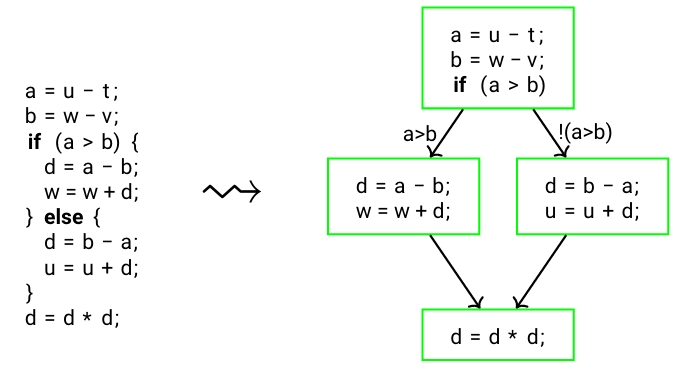
\includegraphics[width=1\textwidth]{Images/Contro-Flow Graph Example.jpeg}
\end{figure}
Path through CFG(P) from the \red{initial} to an \red{exit} node represents \red{one execution sequence} of P

\subsubsection*{Complex Control Flow}
\blue{Loops}

\begin{figure}[h]
    \centering
    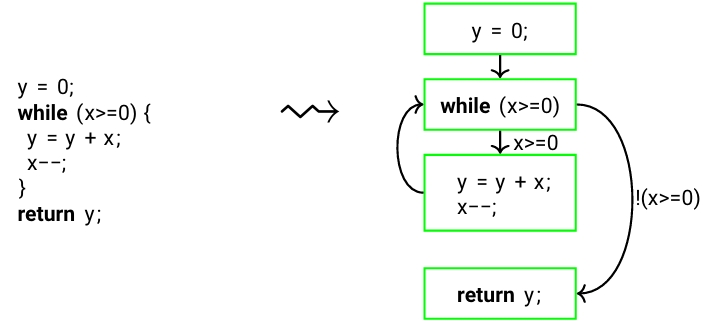
\includegraphics[width=0.9\textwidth]{Images/Loops.jpeg}
\end{figure}

Loop guard \red{not} in initial basic block: can be \red{independently} executed \\
\clearpage
\blue{Exeptions} 
\begin{figure}[h]
    \centering
    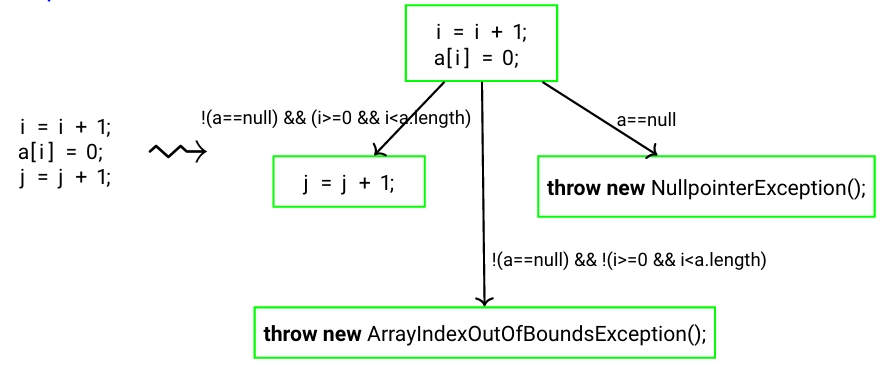
\includegraphics[width=0.9\textwidth]{Images/Exceptions.jpeg}
\end{figure}

Basic block ends, whenever a statement can throw an \red{exception} (branching) (Example also illustrates CFG with \red{multiple exit nodes})

\subsubsection*{Variant: Explicit Initial/Exit Nodes}
\begin{figure}[h]
    \centering
    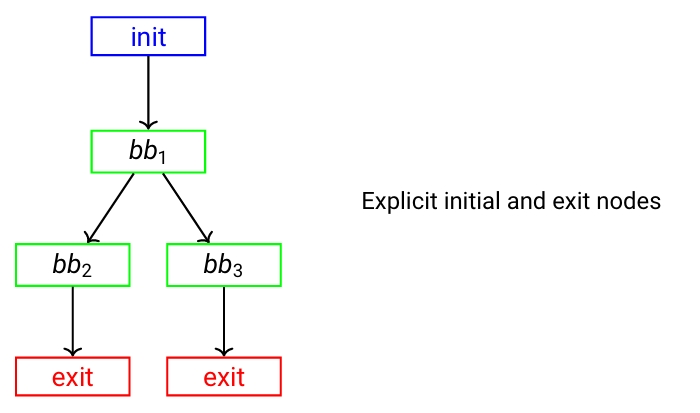
\includegraphics[width=0.9\textwidth]{Images/exit nodes.jpeg}
\end{figure}
\clearpage
\begin{figure}[h]
    \centering
    \includegraphics[width=0.9\textwidth]{Images/Variant: Explicit Initial-Exit Nodes.jpeg}
\end{figure}
\subsubsection*{Removal of Inactive Edges}
\begin{figure}[h]
    \centering
    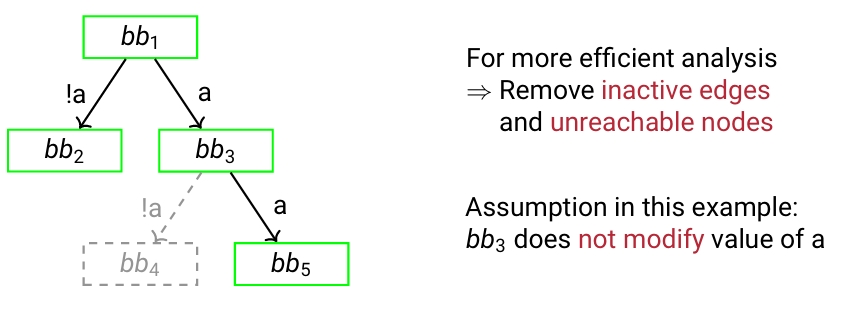
\includegraphics[width=0.9\textwidth]{Images/Removal of Inactive Edges.jpeg}
\end{figure}
\clearpage
\subsection{Code Metric: Cyclomatic Complexity}
\begin{figure}[h]
    \centering
    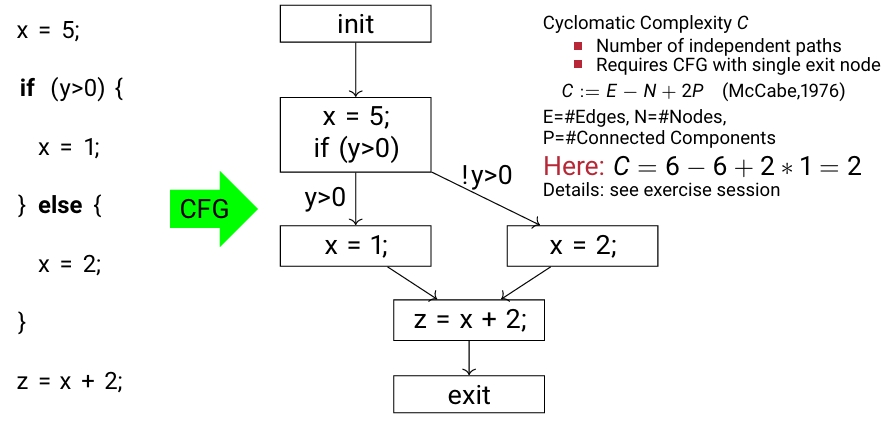
\includegraphics[width=0.9\textwidth]{Images/Cyclomatic Complexity.jpeg}
\end{figure}
\begin{defBox}
    \fatsf{Heuristics:} C>10 \red{rethink} design/coding to reduce complexity
\end{defBox}
\subsection{Code Measure: Class and Interface Coupling}
\begin{defBox}[title=Coupling...]
    ...indicates the amount of \red{dependence} between classes and packages
\end{defBox}
\begin{defBox}[title=Definition(Class and Interface Coupling)]
    A class or interface C is \red{coupled to a} class or interface D if C requires D directly or indirectly
\end{defBox}
\begin{itemize}
    \item A class that depends on 2 other classes has a \red{looser} coupling than a class that depends on 8 other classes
\end{itemize}
\begin{defBox}
    Like cyclomatic complexity, coupling is an \blue{evaluative} principle
\end{defBox}
\subsection{Common Occurences of Coupling in OOP}
\begin{itemize}
    \item Type X has an \red{attribute} that refers to a type Y
    \begin{codeBlock}{}
        class X {private Y y = ...}
        class X {private Y[] y = ...}
    \end{codeBlock}
    \item Type X contains a \red{(sub-)expression} of a type Y
    \begin{codeBlock}{}
        class X {private Object o = new Y();}
        class X {void m(){... if (o instanceof Y) ...}}
        class X {void m(){... x = o.a.count + 3; ...}} //where o.a is of type Y
    \end{codeBlock}
    \item A type X object \red{calls} methods of a type Y
    \begin{codeBlock}{}
        class X {void g(){Y.f();}}
        where class Y {static void f() {...}}
    \end{codeBlock}
    \item Type X \red{has a method that references} an instance of type Y (as method parameter, local variable, return type, ...)
    \begin{codeBlock}{}
        class X {X(Y y) {...}}
        class X {Y f() {...}}
        class X {void g() {Y y = ...;}}
        class X {void h() {Object o = new Y();}}
    \end{codeBlock}
    \item Type X is a \red{subtype} of type Y
    \begin{codeBlock}{}
        class Y {...}
        class X extends Y {...}
        class X implements Y {...}
    \end{codeBlock}
\end{itemize}
\subsection{Coupling in Java: An example}
\begin{codeBlock}{}
    package de.tud.simpletexteditor;
    import java.awt.event.ActionEvent;
    import java.awt.event.ActionListener;
    public class QuitAction implements ActionListener extends Object{
        @Override
        public void actionPerformed(ActionEvent e){
            System.exit(0);
        }
    }
\end{codeBlock}
Class \blue{QuitAction} is coupled directly with ...
\begin{itemize}
    \item ActionListener
    \item ActionEvent
    \item java.lang.Override
    \item java.lang.System
    \item java.lang.Object (any class in Java without an extends clause inherits directly from java.lang.Object)
\end{itemize}
\subsection{Design Principle: Avoid Tight Coupling, Avoid Very Loose Coupling}
\begin{infoBox}[title=Design-Prinzip: Vermeidung von starker Kopplung (aber nicht zu locker)]
    \begin{enumerate}
        \item \fatsf{Definition:}
        \begin{itemize}
            \item \fatsf{Starke Kopplung:} Klassen oder Komponenten sind stark voneinander abhängig, was dazu führt, dass Änderungen an einer Klasse viele anderen betreffen
            \item \fatsf{Lockere Kopplung:} Klassen/Komponenten haben minimale Abhängigkeiten und können unabhängig voneinander agieren, was Modularität und Wiederverwendbarkeit verbessert
        \end{itemize}
    \end{enumerate}
\end{infoBox}
\begin{infoBox}[title=Warum starke Kopplung problematisch ist:]
    \begin{itemize}
        \item \fatsf{Änderungskaskaden:} Änderungen an einer Klasse erfordern Änderungen in allen abhängigen Klassen
        \item \fatsf{Schwierige Verständlichkeit:} Stark gekoppelte Klassen sind schwer isoliert zu verstehen, da ihre Funktion von anderen abhängt
        \item \fatsf{Geringe Wiederverwendbarkeit:} Stark gekoppelte Klassen sind schwer in anderen Projekten einsetzbar, da immer auch die abhängigen Klassen benötigt werden
        \item \fatsf{Niedrige Modularität:} Starke Abhängigkeiten erschweren es, Teile des Systems zu isolieren und modular zu gestalten
    \end{itemize}
\end{infoBox}
\begin{infoBox}[title=Warum zu lockere Kopplung ebenfalls problematisch ist:]
    \begin{itemize}
        \item \fatsf{Grundprinzip der objektorientierten Programmierung (OOP):} OOP setzt auf Objekte, die miteinander kommunizieren. Zu wenig Kopplung führt zu isolierten Objekten, die nicht gut zusammenarbeiten
        \item \fatsf{Zentralisierung:} Übermäßig lockere Kopplung kann dazu führen, dass wenige \enquote{aktive} Objekte die gesamte Arbeit übernehmen müssen, was das System ineffizient und schwer wartbar macht
    \end{itemize}
\end{infoBox}
\begin{infoBox}[title=Der optimale Ansatz]
    \begin{itemize}
        \item Ziel ist eine \fatsf{lockere Kopplung}, die:
        \begin{itemize}
            \item Eine klare Kommunikation zwischen Klassen/Komponenten ermöglicht
            \item Klassen voneinander unabhängig macht, sodass sie leichter gewartet und wiederverwendet werden können
            \item Zentralisierte Arbeitslasten oder ineffiziente Strukturen vermeidet
        \end{itemize}
        \item \fatsf{Praktische Umsetzung:}
        \begin{itemize}
            \item Verwenden von \fatsf{Design-Patterns} wie Dependency Injection, Schnittstellen (Interfaces) oder das Observer-Pattern, um die richtige Balance zwischen Kopplung und Unabhängigkeit zu finden
        \end{itemize}
    \end{itemize}
\end{infoBox}
\subsection{Tight Coupling vs Loose Coupling}
\begin{defBox}
    Tight coupling to stable design elements and libraries is not a problem by itself (It still depends on the kind of elements to which it is coupled)
\end{defBox}
\begin{defBox}[title=Warning:]
    The quest for loose coupling to achieve reusability for a (hypothetical!) project may lead to \red{unnecessary complexity}\\
    Unwarranted decoupling can be one source of undue \red{class proliferation}: (\enquote{Ausuferung})\\
    Too many classes for the size of a given problem
\end{defBox}
\begin{infoBox}
    Starke Kopplung ist akzeptabel, wenn sie auf stabile, bewährte Elemente abzielt. Eine übermäßige Entkopplung hingegen kann zu unnötiger Komplexität und ineffizientem Design führen. Ziel ist ein ausgewogenes Verhältnis zwischen Kopplung und Entkopplung, das die tatsächlichen Anforderungen des Systems widerspiegelt
\end{infoBox}
\subsection{Class Proliferation: Classes vs. Object Roles}
\begin{defBox}[title=Two ways to model behavior]
    \red{As Class} with own attributes and operations\\
    \red{As Role} of an existing class, i.e. association\\
    \blue{When to create dedicated classes?}
\end{defBox}
\begin{infoBox}[title=Verhalten als eigene Klasse modellieren]
    \begin{itemize}
        \item \fatsf{Beschreibung:} Eine Klasse wird erstellt, die ihre eigenen Attribute und Operationen definiert
        \item \fatsf{Vorteile:}
        \begin{itemize}
            \item \fatsf{Kapselung:} Verhalten und zugehörige Daten sind in einer Einheit gebündelt
            \item \fatsf{Wiederverwendbarkeit:} Die Klasse kann in verschiedenen Kontexten verwendet werden
            \item \fatsf{Klarheit:} Die Klasse hat eine eindeutig definierte Rolle im System
        \end{itemize} 
        \item \fatsf{Wann verwenden?}
        \begin{itemize}
            \item Wenn das Verhalten \fatsf{komplex} ist oder eine \fatsf{unabhängige Existenz} rechtfertigt
            \item Wenn mehrere Objekte dieses Verhalten benötigen und es sich daher lohnt, es zentral zu definieren
            \item Beispiel: Eine Klasse PaymentProcessor für die Verarbeitung von Zahlungen
        \end{itemize}
    \end{itemize}
\end{infoBox}
\begin{infoBox}[title=Verhalten als Rolle einer bestehenden Klasse modellieren]
    \begin{itemize}
        \item \fatsf{Beschreibung:} Verhalten wird einer vorhandenen Klasse als Rolle zugeordnet, oft über eine Assoziation
        \item \fatsf{Vorteile:}
        \begin{itemize}
            \item \fatsf{Effizienz:} Vermeidet die Erstellung unnötiger Klassen
            \item \fatsf{Fokus:} Die bestehende Klasse bleibt zuständig für das Verhalten, das in ihrem Kontext relevant ist
        \end{itemize}
        \item \fatsf{Wann verwenden?}
        \begin{itemize}
            \item Wenn das Verhalten eng mit der vorhandenen Klasse verknüpft ist und keinen eigenständigen Kontext benötigt
            \item Wenn das Verhalten \fatsf{einfach} ist oder auf die Attribute der bestehenden Klasse zugreifen muss
            \item Beispiel: Ein Kunde hat die Rolle eines Bestellers, die durch eine Assoziation modelliert wird
        \end{itemize}
    \end{itemize}
\end{infoBox}
\begin{infoBox}[title=Entscheidungskriterien: Wann neue Klassen erstellen?]
    \begin{enumerate}
        \item \fatsf{Autonomie des Verhaltens:}
        \begin{itemize}
            \item Benötigt das Verhalten eine eigenständige Existenz mit klar abgegrenzten Operationen? $\rightarrow$ \fatsf{Neue Klasse}
        \end{itemize}
        \item \fatsf{Wiederverwendbarkeit:}
        \begin{itemize}
            \item Wird das Verhalten an mehreren Stellen im System benötigt? $\rightarrow$ \fatsf{Neue Klasse}
        \end{itemize}
        \item \fatsf{Komplexität:}
        \begin{itemize}
            \item Ist das Verhalten umfangreich oder kompliziert? $\rightarrow$ \fatsf{Neue Klasse}
        \end{itemize}
        \item \fatsf{Kohäsion:}
        \begin{itemize}
            \item Gehört das Verhalten zur Verantwortung der bestehenden Klasse? $\rightarrow$ \fatsf{Rolle einer Klasse}
        \end{itemize}
        \item \fatsf{Anpassungsfähigkeit:}
        \begin{itemize}
            \item Wird erwartet, dass sich das Verhalten unabhängig von der bestehenden Klasse ändert? $\rightarrow$ \fatsf{Neue Klasse}
        \end{itemize}
    \end{enumerate}
\end{infoBox}
\clearpage
\begin{figure}[h]
    \centering
    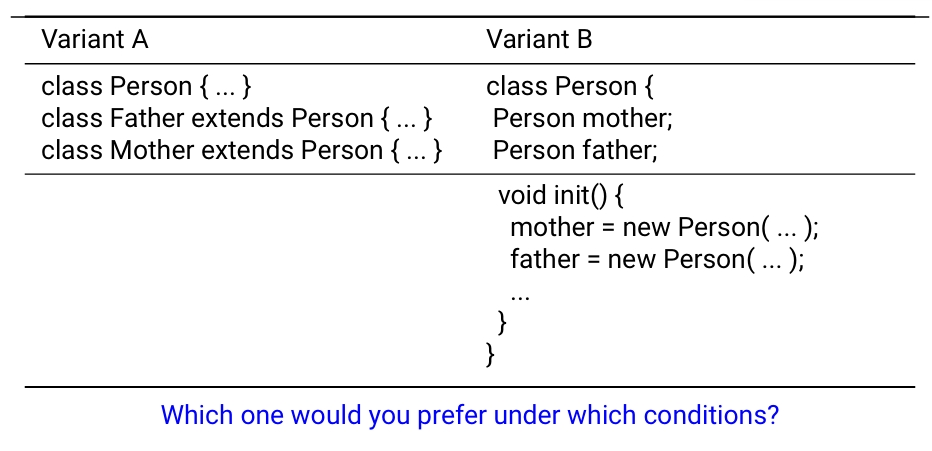
\includegraphics[width=0.9\textwidth]{Images/Class Proliferation.jpeg}
\end{figure}
\begin{itemize}
    \item \red{It depends on the domain model!}\\
    Do Mother/Father exhibit different behavior from Person?
    \item New classes should be warranted by truly \red{different behavior}
\end{itemize}
\subsection{Code Measure: Cohesion}
\begin{defBox}[title=Coheseion ...]
    ...measures the strength of the relation \red{among} elements of a class\\
    \blue{Motivation:}\\
    All operations and data within a class should \enquote{naturally belong} to the concept modelled by the class
\end{defBox}
\begin{defBox}
    Cohesion is an evaluative quality principle
\end{defBox}
\begin{infoBox}[title=Code Measure: Kohäsion (Cohesion)]
    \fatsf{Was ist Kohäsion?}\\
    Kohäsion misst, wie stark die Elemente einer Klasse (Methoden und Attribute) thematisch oder funktional zusammengehören. Eine hohe Kohäsion bedeutet, dass alle Elemente der Klasse sinnvoll miteinander verbunden sind und zu einer klar definierten Aufgabe beitragen
\end{infoBox}
\begin{infoBox}[title=Motivation für Kohäsion]
    \begin{itemize}
        \item \fatsf{Natürliche Zusammengehörigkeit:} Alle Operationen und Daten einer Klasse sollten sich auf das Konzept beziehen, das die Klasse modelliert
        \item \fatsf{Evaluatives Qualitätsprinzip:} Kohäsion wird verwendet, um die Qualität und Verständlichkeit von Klassen zu beurteilen
        \item \fatsf{Verbesserung der Modularität:} Klassen mit hoher Kohäsion sind leichter zu verstehen, zu warten und wiederzuverwenden
    \end{itemize}
\end{infoBox}
\begin{infoBox}[title=Typen von Kohäsion (nach Qualität geordnet)]
    \begin{enumerate}
        \item \fatsf{Zufällige (Coincidental) Kohäsion}
        \begin{itemize}
            \item \fatsf{Beschreibung:} Keine sinnvolle Beziehung zwischen den Elementen einer Klasse
            \item \fatsf{Beispiel:} Eine Klasse enthält Methoden und Daten, die nichts miteinander zu tun haben
            \item \fatsf{Bewertung:} Sehr schlecht. Sollte vermieden werden (außer bei Dienst- oder Utility-Klassen)
        \end{itemize}
        \item \fatsf{Temporale (Temporal) Kohäsion}
        \begin{itemize}
            \item \fatsf{Beschreibung:} Alle Elemente werden zur gleichen Zeit oder in einer bestimmten Reihenfolge ausgeführt
            \item \fatsf{Beispiel:} Initialisierungsmethoden, die nicht zusammenhängen, aber alle beim Start ausgeführt werden
            \item \fatsf{Bewertung:} Schlechte Praxis, da die Elemente keine thematische Verbindung haben
        \end{itemize}
        \item \fatsf{Sequentielle (Sequential) Kohäsion}
        \begin{itemize}
            \item \fatsf{Beschreibung:} Der Output einer Methode ist der Input für eine andere Methode
            \item \fatsf{Beispiel:} Eine Verarbeitungspipeline innerhalb einer Klasse
            \item \fatsf{Bewertung:} Mittel. Es gibt eine Beziehung zwischen den Elementen, aber die Verbindung ist rein sequentiell
        \end{itemize}
        \item \fatsf{Kommunikative (Communicational) Kohäsion}
        \begin{itemize}
            \item \fatsf{Beschreibung:} Alle Methoden der Klasse arbeiten mit denselben Eingabe- oder Ausgabedaten
            \item \fatsf{Beispiel:} Methoden, die verschiedene Operationen auf denselben Daten durchführen, z.B. eine Customer-Klasse mit Zugriff auf Kundendaten
            \item \fatsf{Bewertung:} Gut. Die Methoden teilen sich Daten und haben daher eine klare Verbindung
        \end{itemize}
        \item \fatsf{Funktionale (Functional) Kohäsion}
        \begin{itemize}
            \item \fatsf{Beschreibung:} Alle Elemente einer Klasse tragen dazu bei, eine einzige, klar definierte Verantwortung zu erfüllen
            \item \fatsf{Beispiel:} Eine Klasse PaymentProcessor, die ausschließlich für Zahlungsabwicklungen zuständig ist
            \item \fatsf{Bewertung:} Ideal. Dies ist der angestrebte Zustand
        \end{itemize}
    \end{enumerate}
\end{infoBox}
\subsection{Measuring Cohesion: Lack of Cohesion of Methods (LCOM)}
\begin{infoBox}[title=Was ist LCOM?]
    LCOM (Lock of Cohesion of Methdos) ist ein Indikator für die \fatsf{funktionale Kohäsion} einer Klasse. Es bewertet, wie stark die Methoden einer Klasse miteinander verbunden sind. Ein hoher LCOM-Wert deutet auf \fatsf{geringe Kohäsion} hin, was auf eine suboptimale Klassenstruktur hinweist.
\end{infoBox}
\begin{infoBox}[title=Definition (LCOM nach Li \& Henry)]
    Gegeben:
    \begin{itemize}
        \item C: Eine Klasse mit:
        \begin{itemize}
            \item F: Instanzfelder (Attribute)
            \item M: Methoden (außer Konstruktoren)
        \end{itemize}
    \end{itemize}
    \begin{enumerate}
        \item \fatsf{Graphenrepräsentation:}
        \begin{itemize}
            \item G(M, E): Ein ungerichteter Graph, in dem:
            \begin{itemize}
                \item M die Knoten (Methoden) sind
                \item E die Kanten zwischen Methoden darstellen
            \end{itemize}
            \item Es gibt eine Kante zwischen $m_{1}$ und $m_{2}$, wenn sie ein gemeinsames Feld f $\in$ F verwenden
        \end{itemize}
        \item \fatsf{LCOM-Wert}
        \begin{itemize}
            \item \fatsf{LCOM(C):} Anzaahl der \fatsf{zusammenhängenden Komponenten (Connected Components, CC)} im Graphen G
            \item Wertebereich: \fatsf{LCOM(C)$\in$[0, |M|]}, wobei:
            \begin{itemize}
                \item 0: Hohe Kohäsion (alle Methoden sind verbunden)
                \item |M|: Maximale Zerstreuung (jede Methode ist isoliert)
            \end{itemize}
        \end{itemize}
    \end{enumerate}
\end{infoBox}
\begin{infoBox}[title=Interpretation]
    \begin{itemize}
        \item \fatsf{Hoher LCOM-Wert:}
        \begin{itemize}
            \item Niedrige Kohäsion. Methoden sind unabhängig und teilen keine gemeinsamen Attribute
            \item Die Klasse könnte in mehrere kleinere Klassen aufgeteilt werden
        \end{itemize}
        \item \fatsf{Niedriger LCOM-Wert:}
        \begin{itemize}
            \item Hohe Kohäsion. Methoden arbeiten eng zusammen und sind durch gemeinsame Attribute verbunden
            \item Die Klasse repräsentiert klar ein Konzept
        \end{itemize}
    \end{itemize}
\end{infoBox}
\begin{infoBox}[title=Probleme und Herausforderungen der Formalisierung]
    \begin{enumerate}
        \item \fatsf{Sondermethoden:}
        \begin{itemize}
            \item Konstruktoren, toString(), hashcode(), und andere Standardmethoden beeinflussen LCOM, obwohl sie oft keine Kohäsionsprobleme darstellen
        \end{itemize}
        \item\fatsf{indirekte (transitive) Aufrufe:}
        \begin{itemize}
            \item Methoden könnten indirekt verbunden sein, was durch die einfach Definition von LCOM nicht erfasst wird
        \end{itemize}
        \item \fatsf{Datenzentrierung:}
        \begin{itemize}
            \item Der Fokus liegt nur auf der gemeinsamen Nutzung von Feldern. Methoden könnten jedoch kohäsiv sein, ohne dieselben Felder zu verwenden
        \end{itemize}
        \item \fatsf{Werteinterpretation:}
        \begin{itemize}
            \item Ein hoher Wert ist nicht immer schlecht; es hängt von der Funktionalität der Klasse ab
        \end{itemize}
    \end{enumerate}
\end{infoBox}
\subsection{Cohesion in Java: Example}
\begin{codeBlock}{}
    public class SimpleLinkedList{
        private final int value;
        private final SimpleLinkedList tail;
        public SimpleLinkedList(int v, SimpleLinkedList t){
            this.value = v; this.tail = t;
        }
        //methods
        public int geValue(){return value;}
        public SimpleLinkedList getTeil(){return tail;}
        public boolean contains(int searchFor){
            if (searchFor == value){return true;}
        return tail == null ? false : tail.contains(searchFor);
        }
    }
\end{codeBlock}
\begin{center}
    M = \{getValue, getTail, contains\}
\end{center}
\begin{figure}[h]
    \centering
    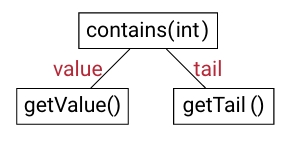
\includegraphics[width=0.5\textwidth]{Images/Cohesion in Java.jpeg}
\end{figure}
\begin{center}
    \begin{itemize}
        \item LCOM = 1 (of 3)
        \item High cohesion
        \item Maximal cohesion for intended behaviour
    \end{itemize}
\end{center}
\begin{codeBlock}{}
    import java.awt.Color;
    abstract class AbstractColorableFigure implements Figure{
        private Color lineColor = Color.BLACK;
        private Color fillColor = Color.WHITE;
        public Color getLineColor(){return lineColor;}
        public void setLineColor(Color c){lineColor = c;}
        public Color getFillColor(){return fillColor;}
        public void setFillColor(Color c){this.fillColor = c;}
    }
\end{codeBlock}
\begin{figure}[h]
    \centering
    \includegraphics[width=0.5\textwidth]{Images/Cohesion in Java: Example 2.jpeg}
\end{figure}
\begin{center}
    \begin{itemize}
        \item LCOM = 2 (of 4)
        \item Relatively low cohesion
        \item Reason:
        \begin{itemize}
            \item Conceptually independent attributes
            \item getter/setter methods
        \end{itemize}
        \item How to improve cohesion?
        \begin{itemize}
            \item Factor out common functionality from subclasses relted to color
            \item Maybe ColorableFigure is not a good abstraction
            \item Might be justifiable if several impementing subclasses exist
        \end{itemize}
    \end{itemize}
\end{center}
\subsection{Design Principle: Avoid Low Cohesion}
Classes with low cohesion are \red{undesirable}:
\begin{itemize}
    \item Hard to \red{comprehend}
    \item Hard to \red{reuse}
    \item Hard to \red{maintain} (easily affected by change)
    \item Typically represent \red{too coarse-grained abstraction}
    \item Often take responsibility that should have been \red{delegated}
\end{itemize}
\begin{defBox}
    \red{Observation:} Classes with high cohesion can often be described in a single sentence
\end{defBox}
\section{Part III: Responsibility-Driven Design}
\subsection{Designing Software Objects}
\subsubsection*{Responsibility-Driven Design}
\begin{defBox}
    A systematic approach to think about the \red{design} of software objects and components in terms of \red{responsiblities}, \red{roles} and \red{collaborations}
\end{defBox}
\begin{figure}[h]
    \centering
    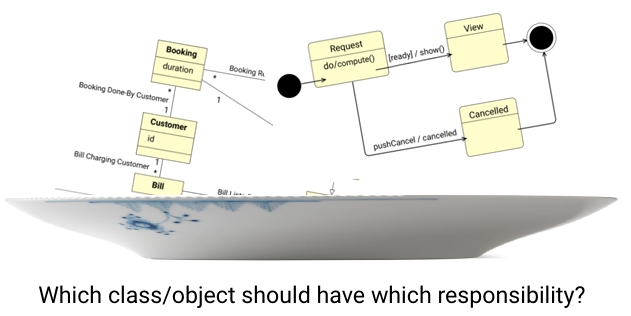
\includegraphics[width=1\textwidth]{Images/Responsibility.jpeg}
\end{figure}
\subsection{Responsibilities}
\begin{infoBox}[title=Definition und Bedeutung von Verantwortlichkeiten]
    \begin{itemize}
        \item Eine \fatsf{Verantwortlichkeit} repräsentiert eine Aufgabe oder Funktion, die einer Klasse in einem Softwaredesign zugewiesen wird
        \item Jede Verantwortlichkeit stellt eine mögliche \fatsf{Änderungsachse} dar:
        \begin{itemize}
            \item Wenn sich Anforderungen ändern, führen diese Änderungen oft zu einer Anpassung der entsprechenden Verantwortlichkeiten in den Klassen
        \end{itemize}
        \item Klassen mit \fatsf{mehreren Verantwortlichkeiten} haben \fatsf{mehrere Gründe}, sich zu ändern, was die Wartbarkeit und Stabilität des Codes verringert
    \end{itemize}
\end{infoBox}
\begin{infoBox}[title=Zitat von Robert C. Martin]
    \begin{itemize}
        \item \enquote{Jede Verantworltlichkeit ist eine Achse der Veränderung}
        \item \fatsf{Implikation:}
        \begin{itemize}
            \item Klassen sollten so entworfen sein, dass sie möglichst wenige Verantwortlichkeiten tragen. Dies minimiert die Notwendigkeit, mehrere Änderungen an einer Klasse vorzunehmen, wenn sich Anforderungen ändern
        \end{itemize}
    \end{itemize}
\end{infoBox}
\begin{infoBox}[title=Zuweisung von Verantwortlichkeiten]
    \begin{itemize}
        \item Das \fatsf{Zuweisen von Verantwortlichkeiten} ist ein zentraler Schritt im Code-Design
        \item Ziel: Klassen so gestalten, dass sie \fatsf{klar definiert und abgegrenzte Verantwortlichkeiten} haben
        \item \fatsf{Tools und Techniken zur Unterstützung:}
        \begin{itemize}
            \item \fatsf{Entwurfsmuster} (z.B. Singleton, Factory)
            \item \fatsf{Designprinzipien} (z.B. SOLID-Prinzipien)
            \item \fatsf{Idiome} (sprachspezifische Konventionen und Muster)
        \end{itemize}
    \end{itemize}
\end{infoBox}
\begin{infoBox}[title=Responsibility-Driven Design (RDD)]
    \begin{itemize}
        \item Im \fatsf{Responsibility-Driven Design} (RDD) liegt der Fokus auf der \fatsf{Definition von Verantwortlichkiten} und der Zuweisung dieser an Objekte
        \item \fatsf{Merkmale von RDD:}
        \begin{itemize}
            \item Softwareobjekte werden nicht nur als Datencontainer betrachtet, sondern als Einheiten, die \fatsf{Verantwortlichkeiten übernehmen}
            \item Verantwortlichkeiten können in zwei Kategorien unterteilt werden:
            \begin{enumerate}
                \item \fatsf{Was ein Objekt weiß} (Daten oder Zustände, die ein Objekt speichert)
                \item \fatsf{Was ein Objekt tut} (Funktionen oder Aktionen, die ein Objekt ausführt)
            \end{enumerate}
        \end{itemize}
        \item Verantwortlichkeiten werden in der \fatsf{Objektdesign-Phase} festgelegt, wobei Klassen und ihre Interaktionen im Mittelpunkt stehen
    \end{itemize}
\end{infoBox}
\subsection{Types of Responsibilities}
\begin{infoBox}[title=Grundtypen von Verantwortlichkeiten]
    \begin{enumerate}
        \item \fatsf{Doing Responsibilities (Tätigkeitsverantwortlichkeiten)}
        \begin{itemize}
            \item Diese beziehen sich auf die \fatsf{Ausführung von Aktionen}
            \item Beispiele für Tätigkeiten:
            \begin{itemize}
                \item Eine Aufgabe direkt ausführen (z.B. Berechnungen durchführen, Objekte erstellen)
                \item Eine Aktion in anderen Objekten initiieren
                \item Aktivitäten in anderen Objekten \fatsf{steuern} und \fatsf{koordinieren}
            \end{itemize}
            \item \fatsf{Beispiel:}
            \begin{itemize}
                \item Ein \fatsf{Rechnungsobjekt} (Bill) ist dafür verantwortlich, die Gesamtsumme der Rechnung zu berechnen
            \end{itemize}
        \end{itemize}
        \item \fatsf{Knowing Responsibilities (Wissensverantwortlichkeiten):}
        \begin{itemize}
            \item Diese beziehen sich auf das \fatsf{Wissen} eines Objekts und die Fähigkeit, Informationen bereitzustellen
            \item Arten von Wissen:
            \begin{itemize}
                \item \fatsf{Privates, gekapseltes Wissen} (z.B. interne Daten oder Attribute der Klasse)
                \item \fatsf{Beziehungen zu anderen Objekten} (z.B. Kenntnis über verbundene Objekte)
            \end{itemize}
            \item \fatsf{Beispiel:}
            \begin{itemize}
                \item Ein \fatsf{Auto-Objekt} (Car) ist dafür verantwortlich, die gefahrene Strecke zu kennen und bereitzustellen
            \end{itemize}
        \end{itemize}
    \end{enumerate}
\end{infoBox}
\subsection{Relation between Responsibilities and Methods}
\begin{infoBox}[title=Verantwortlichkeiten]
    \begin{itemize}
        \item Beschreiben \fatsf{höherwertige Aufgaben} oder Verpflichtungen, die eine Klasse oder ein Objekt innerhalb eines Softwaresystems übernhemen soll
        \item Eine Verantwortlichkeit kann:
        \begin{itemize}
            \item Durch eine einzige Methode in einem Objekt erfüllt werden
            \item Mehrere Methoden in einem Objekt erfordern
            \item Viele Methoden in mehreren Objekten einbeziehen
        \end{itemize}
        \item Verantwortlichkeiten sind \fatsf{konzeptionell} und dienen als Leitlinie für die Implementierung eines Verhaltens im System
    \end{itemize}
\end{infoBox}
\begin{infoBox}[title=Methoden]
    \begin{itemize}
        \item Sind die \fatsf{konkrete Implementierung} einer Verantwortlichkeit
        \item Sie definieren die spezifischen Aktionen, die ein Objekt ausführt, um seine Verantwortlichkeiten zu erfüllen
        \item Beispiel:
        \begin{itemize}
            \item \fatsf{Verantwortlichkeit:} \enquote{Verwalten einer Datenbankverbindung}
            \item \fatsf{Methode:} connect(), disconnect(), executeQuery()
        \end{itemize}
    \end{itemize}
\end{infoBox}
\begin{infoBox}[title=Wichtige Punkte]
    \begin{enumerate}
        \item \fatsf{Granularität von Verantwortlichkeiten:}
        \begin{itemize}
            \item \fatsf{Fein granulierte Verantwortlichkeiten} benötigen oft wenige Methoden (z.B. das Erstellen einer Rechnung)
            \item \fatsf{Grob granulierte Verantwortlichkeiten} können sich über viele Klassen und Methoden erstrecken (z.B. Zugriff auf eine Datenbank)
        \end{itemize}
        \item \fatsf{Verantwortlichkeiten $\neq$ Methoden:}
        \begin{itemize}
            \item Eine Verantwortlichkeit kann auf viele Methoden oder sogar auf mehrere Objekte verteilt sein
        \end{itemize}
    \end{enumerate}
\end{infoBox}
\subsection{Assigning Responsibilities to Mutiple Objects}
\begin{infoBox}[title=Verantwortlichkeiten auf mehrere Objekte verteilen]
    Bei der Zuweisung von Verantwortlichkeiten gibt es:
    \begin{itemize}
        \item \fatsf{Viele mögliche Ansätze}, was zu unterschiedlichen Designs führen kann:
        \begin{itemize}
            \item \fatsf{Gute Designs:} Wartbar, verständlich, wiederverwendbar und erweiterbar
            \item \fatsf{Schlechte Designs:} Fragile Systeme, die schwer zu warten und zu verstehen sind
        \end{itemize}
        \item Designprinzipien und Muster helfen, Verantwortlichkeiten \fatsf{effizient zuzuweisen}
    \end{itemize}
\end{infoBox}
\begin{infoBox}[title=Strategien für die Zuweisung von Verantwortlichkeiten]
    \begin{enumerate}
        \item \fatsf{Designprinzipien einhalten:}
        \begin{itemize}
            \item \fatsf{Single Responsibility Principle (SRP):} Jede Klasse sollte genau eine Verantwortlichkeit haben
            \item \fatsf{Kapselung (Encapsulation):} Daten und Methoden, die zusammengehören, sollten in einer Klasse bleiben
            \item \fatsf{Hohe Kohäsion, niedrige Kopplung:} Klassen sollten stark zusammenhängend sein, aber möglichst unabhängig von anderen
        \end{itemize}
        \item \fatsf{Designmuster nutzen:}
        \begin{itemize}
            \item Aufgaben an geeignete Objekte delegieren (z.B. Factory für die Objekterstellung, Repository für Datenbankzugriffe)
        \end{itemize}
        \item \fatsf{Wartbarkeit berücksichtigen:}
        \begin{itemize}
            \item Vermeiden, dass Objekte zu viele Verantwortlichkeiten übernehmen
            \item Verantwortlichkeiten logisch zuweisen, um Wiederverwendbarkeit zu fördern
        \end{itemize}
    \end{enumerate}
\end{infoBox}
\section{Part IV: More Design Principles}
\subsection{The Single Responsibility Principle (SRP)}
\enquote{A class should have only one reason to change}\\
\red{A responsibility is usually the primary reason for change}\\
$\Rightarrow$ One responsibility per class (the ideal to achieve)
\section{SRP: Rectangle Example}
\begin{figure}[h]
    \centering
    \includegraphics[width=1\textwidth]{Images/SRP: Rechtangle Example.jpeg}
\end{figure}
Does the Rectangle class follow the \red{Single Responsibility Principle}?\\
The Rectangle class hat \red{multiple} responsibilities:
\begin{itemize}
    \item \red{Calculate} the size of a rectangle: mathematical \red{model}
    \item \red{Render} rectangle on screen: \red{GUI} related functionality
\end{itemize}
Do you see any problems in having multiple responsibilities?
\begin{itemize}
    \item \red{Reuse} of Rectangle hindered b dependency on GUI package (GUI classes have to be deployed along with the Rectangle class)
    \item Any \red{change} in Graphical App causing a change of Rectangle requires to re-test and re-deploy Rectangle in the context of Geometry App
\end{itemize}
\subsection{Refactoring Rectangle to Satisfy SRP}
\begin{figure}[h]
    \centering
    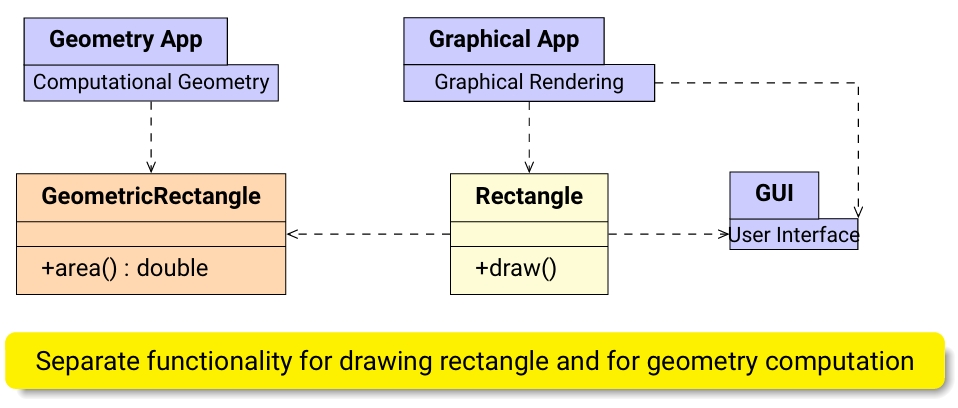
\includegraphics[width=1\textwidth]{Images/Refactoring Rectangle to Satisfy SRP.jpeg}
\end{figure}
\subsection{Collboration of Two Or More Classes}
\blue{Even if SRP is realized, not always clear, where to place a responsibility}
\begin{defBox}
    Designing a policy that requires \red{collaboration} of multiple classes
\end{defBox}
\begin{figure}[h]
    \centering
    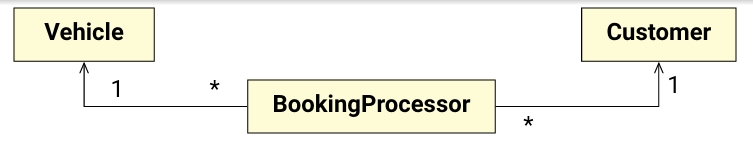
\includegraphics[width=1\textwidth]{Images/Collaboration of Two or More Classes.jpeg}
\end{figure}
\begin{itemize}
    \item \red{Vehicle:} Static Information about vehicle objects: number plate, verhicle class, most recent service, etc.
    \item \red{Customer:} Static information about customer: customer id, name, adress, allowed vehicle classes, etc.
    \item \red{BookingProcessor:} Static \& dynamic information about \red{one} requested booking: which vehicle, duration, who made it, etc.
\end{itemize}
\subsubsection*{Example}
\begin{defBox}[title=Task]
    Implement a check (\blue{checkPermision}) in BookingProcessor whether a customer is allowed to drive the chosen vehicle
\end{defBox}
\begin{defBox}[title=First design]
    \begin{enumerate}
        \item BookingProcessor queries Customer for allowed vehicle categories (calls \\ \blue{possibleCategories=customer.getVehicleCategories()})
        \item BookingProcessor passes vehicle categories to the chosen vehicle for checking (calls \\\blue{isPermitted=vehicle.checkPermission(possibleCategories)})
        \item BookingProcessor decides on outcome whether to continue processing or to reject the request
    \end{enumerate}
\end{defBox}
\begin{defBox}[title=Second design]
    \begin{enumerate}
        \item BookingProcessor queries Vehicle for vehicle categories (calls \blue{vehicleCategory=vehicle.getVehicleCategory()})
        \item BookingProcessor passes vehicle category to customer for checking (calls \\ \blue{isPermitted=customer.checkPermission(vehicleCategory))})
        \item BookingProcessor decides on outcome whether to continue processing or to reject the request
    \end{enumerate}
\end{defBox}
\begin{defBox}[title=Third design]
    \begin{enumerate}
        \item BookingProcessor queries Customer for allowed vehicle categories (calls \\ \blue{possibleCategories=customer.getVehicleCategories()})
        \item BookingProcessor queries Vehicle for vehicle category (calls \blue{vehicleCategory=vehicle.getVehicleCategory()})
        \item BookingProcessor implements check itself, hence, calls \blue{isPermitted=checkPermission(possibleCategories, vehicleCategory)}
        \item BookingProcessor decides on outcome whether to continue processing or to reject the request
    \end{enumerate}
\end{defBox}
\subsection{Delegation vs. Inheritance}
\begin{infoBox}[title=Delegation vs. Vererbung]
    Die Wahl zwischen Delegation und Vererbung ist ein entscheidender Designaspekt in der objektorientierten Programmierung. Hier ein Überblick über die beiden Ansätze, ihre Vor- und Nachteile sowie Richtilinien, wann welcher Ansatz sinnvoll ist.
\end{infoBox}
\begin{infoBox}[title=Vererbung]
    \fatsf{Definition:}
    \begin{itemize}
        \item Eine Klasse erbt von einer anderen Klasse
        \item Die abgeleitete Klasse übernimmt Attribute und Methoden der Basisklasse und kann diese erweitern oder überschreiben
    \end{itemize}
    \fatsf{Vorteile:}
    \begin{enumerate}
        \item \fatsf{Wiederverwendbarkeit:} Code der Basisklasse kann in Unterklassen direkt genutzt werden
        \item \fatsf{Einfache Implementierung:} Die Syntax (extends in Java) ist direkt und etabliert
        \item \fatsf{Konsistenz:} Alle Unterklassen teilen die gleiche Basislogik
    \end{enumerate}
    \fatsf{Nachteile:}
    \begin{enumerate}
        \item \fatsf{Unnatürliche Beziehungen:}
        \begin{itemize}
            \item Führt oft zu einer \enquote{ist-ein} Beziehung, auch wenn eine \enquote{hat-ein} Beziehung passender wäre
            \item Beispiel: Ein \fatsf{Kunde} ist nicht natürlich eine \fatsf{Authentifizierungsinstanz} sondern benötigt sie
        \end{itemize}
        \item \fatsf{Tiefer Vererbungsbaum:}
        \begin{itemize}
            \item Erhöht Komplexität und Wartung
            \item Kann zu fragile base class problem führen: Änderungen an der Basisklasse betreffen ungewollt alle Unterklassen
        \end{itemize}
        \item \fatsf{Verletzung des Single Responsibility Principle (SRP):}
        \begin{itemize}
            \item Eine Klasse übernimmt potenziell Verantwortlichkeiten, die sie nicht direkt betreffen
        \end{itemize}
        \item \fatsf{Unflexibel zur Laufzeit:}
        \begin{itemize}
            \item Vererbungsbeziehungen sind statisch und können nicht dynamisch geändert werden
        \end{itemize}
    \end{enumerate}
\end{infoBox}
\begin{infoBox}[title=Delegation]
    \fatsf{Definition:}
    \begin{itemize}
        \item Ein Objekt delegiert Aufgaben an ein anderes Objekt, das die erforderliche Funktionalität bereitstellt
        \item Beispiel: Statt dass die Klasse \fatsf{Customer} Authetifizierung direkt implementiert, ntutzt sie ein \fatsf{Authentication}-Objekt, um die Authentifizierung zu delegieren
    \end{itemize}
    \fatsf{Vorteil:}
    \begin{enumerate}
        \item \fatsf{Hohe Flexibilität:}
        \begin{itemize}
            \item Delegierte Objekte können zur Laufzeit geändert oder dyamisch erzeugt werden
        \end{itemize}
        \item \fatsf{Bessere Kapselung:}
        \begin{itemize}
            \item Jede Klasse bleibt auf ihre Kernaufgabe fokussiert, was das \fatsf{SRP} unterstützt
        \end{itemize}
        \item \fatsf{Leichte Wartbarkeit:}
        \begin{itemize}
            \item Änderungen an delegierten Code betreffen nur das Delegationsobjekt, nicht die Hauptklasse oder andere Delegierende
        \end{itemize}
        \item \fatsf{Geringere Kopplung:}
        \begin{itemize}
            \item Klassen sind weniger stark auseinander gebunden als bei Vererbung
        \end{itemize}
    \end{enumerate}
    \fatsf{Nachteile:}
    \begin{enumerate}
        \item \fatsf{Komplexere Implementierung}
        \begin{itemize}
            \item Zusätzliche Objekte und Interaktionen müssen eingeführt werden
        \end{itemize}
        \item \fatsf{Kein dedizierter Sprachsupport}
        \begin{itemize}
            \item Delegation muss manuell implementiert werden, während Vererbung direkt durch die Sprache unterstützt wird
        \end{itemize}
    \end{enumerate}
\end{infoBox}
\subsection{Implementing Delegation}
\begin{figure}[h]
    \centering
    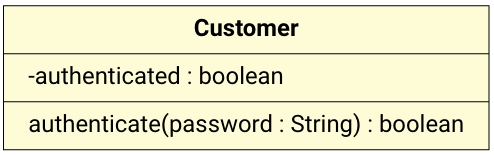
\includegraphics[width=1\textwidth]{Images/Implementing Delegation.jpeg}
\end{figure}
\begin{codeBlock}{}
    public class Customer{
        private boolean authenticated;
        public boolean authenticate(String password){
            authenticated = (Authentication.getAuthenticationToken(this)).authenticate(password);
            return authenticated;
        }
    }
\end{codeBlock}
\begin{infoBox}
    Hier:
    \begin{itemize}
        \item \fatsf{Customer} delegiert die Authentifizierung an ein \fatsf{Authentication}-Objekt
        \item Dadurch bleibt \fatsf{Customer} schlank und übernimmt nur die Aufgae, das Ergebnis zu speichern und zurückzugeben
    \end{itemize}
\end{infoBox}
\subsection{When to Use Delegation, When Inheritance?}
\begin{defBox}
    Inheritance must extend existing functionality \red{organically}
\end{defBox}
\blue{In many cases, delegation is preferable:}
\begin{itemize}
    \item Less intrusive on overall design, more focused
    \item Delegate can be changed/determined at runtime
\end{itemize}
\red{But:} No dedicated syntax like \fatsf{extends} in Java
\begin{defBox}[title=But isn't inheritance the essence of OO design?]
    No! The essence of OO is object \red{communication}, not inheritance!
\end{defBox}
\section{Part V: Encapsulation}
\subsection{Programming to Interfaces}
\begin{defBox}[title=Interface Concept]
    An \red{interface} declares the \blue{method signatures} and \blue{public constants} of its implementing classes
    \begin{itemize}
        \item Interfaces provide \red{independence} of functionality from implementation
    \end{itemize}
\end{defBox}
\begin{defBox}
    Always \enquote{\red{program to interfaces}}
\end{defBox}
\begin{defBox}[title=What does this mean?]
    \begin{itemize}
        \item Declare fields, return types, method parameters with \red{interface} type
        \item Do not expose \red{implementation details} in public methods
        \item Declare fields in implementing classes as \red{private}: use getters/setters
    \end{itemize}
\end{defBox}
\clearpage
\subsubsection*{Example}
\begin{figure}[h]
    \centering
    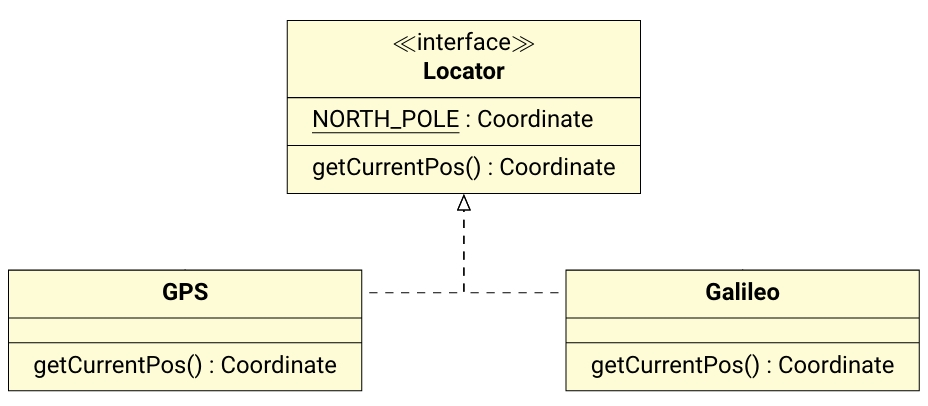
\includegraphics[width=0.9\textwidth]{Images/Programming to Interfaces 1.jpeg}
\end{figure}
\begin{figure}[h]
    \centering
    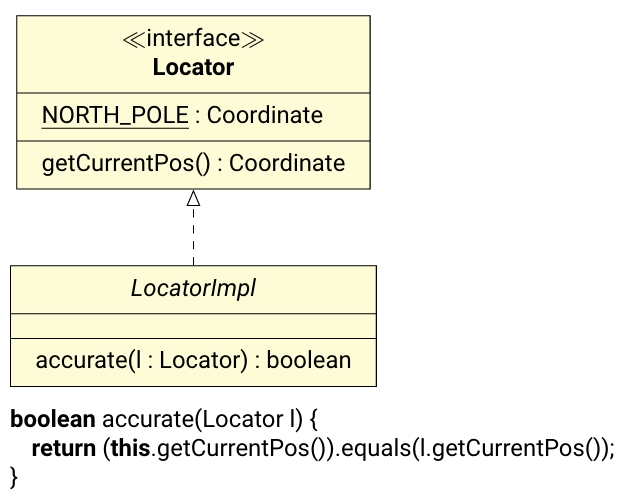
\includegraphics[width=0.6\textwidth]{Images/programmin to Interfaces 2.jpeg}
\end{figure}
\subsection{Programming to Interfaces: Advantages}
\begin{itemize}
    \item Helps to avoid \red{unjustified assumptions} about implementation
    \item Interfaces more \red{stable} than implementations
    \item To change implementation, sufficient to \red{exchange constructor}
    \begin{itemize}
        \item Can factor out implementation-independent code into abstract classes \blue{(as seen)}
        \item Reduces coupling (no dependence on implementing class)
    \end{itemize}
\end{itemize}
\subsection{Field Access}
\begin{defBox}
    \blue{Design principle:} make instance fields of classes \red{never} public
\end{defBox}
\begin{itemize}
    \item Breaks principle of \red{information hiding} and \red{programming to interfaces}:
    \begin{itemize}
        \item No distinction between implementation-specific and public data
        \item Implementation-specific details exposed to clients
    \end{itemize}
    \item \red{Brittle} code once field implementation changes
    \item Fields passed as arguments or aliased: hard to keep track of \red{dependencies} (coupling)
\end{itemize}
\begin{infoBox}
    Die Verletzung von \fatsf{Information Hiding und Programming to Interfaces} hat folgende Auswirkungen:
    \begin{enumerate}
        \item \fatsf{Fehlende Kapselung:} Änderungen in der Implementierung erfordern Änderungen im gesamten Client-Code
        \item \fatsf{Erhöhte Kopplung:} Schwer nachvollziehbare Abhängigkeiten zwischen Klassen entstehen
        \item \fatsf{Instabilität:} Der Code wird anfällig für Fehler und schwer wartbar
        \item \fatsf{Verlust der Kontrolle:} Direkte Manipulation von Feldern oder Objekten unterläuft die Verantwortung der Klasse
    \end{enumerate}
\end{infoBox}
\begin{defBox}[title=How to Access Fields of Other Objects?]
    Provide suitable \red{accessor} methods
    \begin{itemize}
        \item For field of type T named X: \blue{T getX() void setX(T x)}
    \end{itemize}
\end{defBox}
\subsection{Accessor Methods Exposing too Mush}
\begin{figure}[h]
    \centering
    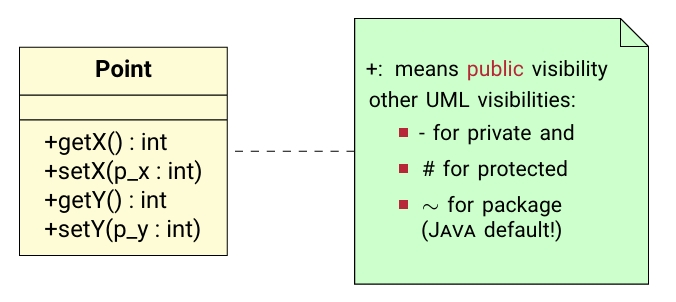
\includegraphics[width=0.6\textwidth]{Images/Point.jpeg}
\end{figure}
\blue{Class Point has public accessor operations}
\begin{itemize}
    \item Are there any problems with the above design of class Point?
    \item Does class Point expose too much implementation details to clients?
\end{itemize}
\begin{defBox}
    Accessor methods do \red{not necessarily} expose implementation details
\end{defBox}
\blue{But there is still an issue - What is it?}
\begin{itemize}
    \item Accessor methods may encourage poor encapsulation of \red{behavior}: Client accessing (x, y)-coordinates of \fatsf{Point} objects might implement behavior of points \red{not provided by} \fatsf{Point}
    \item Encourages misplacing \red{responsibilities}
\end{itemize}
\begin{infoBox}[title=Emfohlene Lösung: Methoden zur Kapselung von Verhalten]
    Anstatt Getter und Setter zu verwenden, sollte die Klasse die relevanten Operationen selbst implementieren, Beispiel:
    \begin{codeBlock}{}
        public class Point {
        private int x;
        private int y;
        // Konstruktor
        public Point(int x, int y) {
            this.x = x;
            this.y = y;
        }
        // Verhalten implementieren
        public void move(int dx, int dy) {
            this.x += dx;
            this.y += dy;
        }
        public double distanceTo(Point other) {
            int dx = this.x - other.x;
            int dy = this.y - other.y;
            return Math.sqrt(dx * dx + dy * dy);
        }
    
        @Override
        public String toString() {
            return "(" + x + ", " + y + ")";
        }
    }
    \end{codeBlock}
\end{infoBox}
\begin{infoBox}[title=Vorteile der verbesserten Kapselung]
    \begin{enumerate}
        \item \fatsf{Encapsulation (Bessere Kapselung):}
        \begin{itemize}
            \item Die Klasse Point ist vollständig verantwortlich für das Verhalten von Punkten
            \item Clients haben keinen direkten Zugriff auf interne Details
        \end{itemize}
        \item \fatsf{Reduced Coupling (Reduzierte Kopplung):}
        \begin{itemize}
            \item Änderungen an der internen Repräsentation von Point (z.B. Umstellung auf Polarkoordination) wirken sich nicht direkt auf den Client aus
        \end{itemize}
        \item \fatsf{Improved Responsibility Assignment (Bessere Verantwortungsverteilung):}
        \begin{itemize}
            \item Verhlaten wie Verschiebung oder Distanzberechnung bleibt innerhalb der Klasse, die die Daten enthält
        \end{itemize}
    \end{enumerate}
\end{infoBox}
\subsection{Accessor Methods for Private Fields: Generally Discourage?}
\begin{infoBox}
    Zugriffsmethoden (Getter und Setter) werden oft kritisiert, da sie interne Implementierungsdetails offenlegen und damit die Kapselung verletzen können. Dennoch gibt es bestimmte Szenarien, in denen sie gerechtfertigt und sogar notwendig sind. Hier eine Erklärung, wann und warum Zugriffsmethoden sinnvoll eingesetzt werden können:
\end{infoBox}
\begin{infoBox}[title=Notwendig für die Benutzeroberfläche (UI)]
    \begin{itemize}
        \item \fatsf{Szenario:} Wenn eine Klasse Daten repräsentiert, die in der Benutzeroberfläche angezeigt werden müssen, können Zugriffsmethoden einen kontrollierten Zugang zu den zugrunde liegenden Daten ermöglichen
        \item \fatsf{Grund:} Die UI benötigt oft die Rohdaten (z.B. Namen, Alter oder Koordination), um sie darzustellen, ohne direkt auf die interne Logik der Klasse zuzugreifen
        \item \fatsf{Beispiel:}
        \begin{codeBlock}{}
            public class User{
                private String name;
                public String getName(){
                    return name;
                }
            }
        \end{codeBlock}
        \begin{itemize}
            \item Die Methode getName ermöglicht der UI, den Namen des Nutzers anzuzeigen, ohne Zugriff auf die Implementierungsdetails der Klasse zu geben
        \end{itemize}
    \end{itemize}
\end{infoBox}
\begin{infoBox}[title=Durchsetzung von Regeln oder Richtlinien]
    \begin{itemize}
        \item \fatsf{Szenario:} Wenn eine Klasse bestimmte Regeln, Validierungen oder Richtlinien (z.B. Wertebereich oder berechnet Werte) implementieren muss, können Zugriffsmethoden diese Regeln durchsetzen
        \item \fatsf{Grund:} Zugriffsmethoden bieten eine kontrollierte Möglichkeit, Daten zu validieren oderzu verändern, ohne die Kapselung zu brechen
        \item \fatsf{Beispiel:}
        \begin{codeBlock}{}
            public class Account {
                private double balance;
                public double getBalance() {
                    return balance;
                }
                public void setBalance(double balance) {
                    if (balance < 0) {
                        throw new IllegalArgumentException("Das Guthaben darf nicht negativ sein.");
                    }
                    this.balance = balance;
                }
            }
        \end{codeBlock}
        \begin{itemize}
            \item Hier stellt die Methode setBalance sicher, dann kein negatives Guthaben erlaubt ist
        \end{itemize}
    \end{itemize}
\end{infoBox}
\begin{infoBox}[title=Statische Container ohne Verhalten]
    \begin{itemize}
        \item \fatsf{Szenario:} Wenn eine Klasse als einfacher Container für zusammengehörige, statische Daten oder Konstanten dient, können Zugriffsmethoden genutzt werden, um die Daten bereitzustellen
        \item \fatsf{Grund:} Die Klasse hat die Aufgabe, Daten zu speichern und bereitzustellen, sodass Zugriffsmethoden hier nicht der Intention widersprechen
        \item \fatsf{Beispiel:}
        \begin{codeBlock}{}
            public class Config {
                private static final String APP_NAME = "MeineApp";
                public static String getAppName() {
                    return APP_NAME;
                }
            }
        \end{codeBlock}
        \begin{itemize}
            \item Die Klasse Config dient als Container für unveränderliche Daten und bietet über Zugriffsmethoden Leserechte
        \end{itemize}
    \end{itemize}
\end{infoBox}
\begin{defBox}
    Make decisions \red{consciously} and be able to \red{justify} them (Not only here!)
\end{defBox}
\section{Applying Design Knowledge: The God Class Problem}
\subsection{The God Class Problem}
\begin{defBox}[title=God Classes]
    One class contains most of the system logic:
    \begin{itemize}
        \item Poorly distributed responsibilities
        \item Not an object-oriented design (collaborating objects)
    \end{itemize}
\end{defBox}
\subsection{Recognizing and Avoiding God Classes}
\begin{defBox}[title=Classes with unclear responsibilities]
    Class failing SRP\\
    \red{Required Action:} Split class and relocate responsibilities
\end{defBox}
\begin{defBox}[title=Classes with low cohesion\, non-communicating classes]
    Classes with methods operating on a small subset of its fields, not with other objects: \red{non-communicating behavior}\\
    \red{Required Action:} Split class and relocate responsibilities
\end{defBox}
\begin{defBox}[title=Uses classes with public field accessors]
    Can indicate that responsibilities are located in wrong class\\
    \red{Required Action:} Redesign interface and relocate responsibilities
\end{defBox}
\subsubsection*{Summary}
\begin{defBox}
    \red{Distribute} responsibilities uniformly among top-level classes in a design - Adherence to design principles reduces likelihood to create god class
\end{defBox}
\begin{defBox}[title=Sometimes design principles need to be traded off]
    Try to model the real world:\\
    \red{Low representational gap} facilitates maintenance and evolution\\
    \blue{But modelling the real world is not as important as the other principles}
\end{defBox}
\begin{defBox}[title=Example(Car)]
    In the real world, a car does not compute its next service interval\\
    In a car sharing system it is conceivable to assign responsibility for this to its corresponding class
\end{defBox}
\subsection{Design Principles}
\subsubsection*{Summary, Part I}
\begin{defBox}
    \begin{itemize}
        \item Avoid tight coupling of classes
        \item Avoid very loose coupling of classes
        \item Justify existence of classes by new behvior - consider roles
        \item Avoid low cohesion of classes
        \item Strive for single responsibility per class
        \item Use inheritance carefully, consider delegation
    \end{itemize}
\end{defBox}
\subsubsection*{Summary, Part II}
\begin{defBox}
    \begin{itemize}
        \item Avoid class proliferation (design too fine-granular)
        \item Program to interfaces
        \item Never make instance fields public, provide accessors if needed
        \item But: Provide only accessors needed for functionality
        \item Distribute functionalities evenly, avoid god classes
    \end{itemize}
\end{defBox}